\section{Výstupní data}

\subsection{Nejkratší cesta}

\subsubsection{Zvolená trasa pro testování: Skořice \texorpdfstring{\(\rightarrow\)}{->} Němčovice}
\textbf{Nejkratší cesta podle} \href{https://mapy.cz/letecka?planovani-trasy&rc=9ezy9xVfEq9efLtxWmgn&rs=muni&rs=muni&ri=58&ri=2029&mrp=%7B%22c%22%3A111%7D&xc=%5B%5D&rwp=1%3B9ew5DxVgNta6jmurcf.jsIc..jMqfITmr-eIZmXQSnxW6EjfHQxW-1g3i-xWg5N&rut=1&x=13.6007336&y=49.7887247&z=11}{\textbf{Mapy.cz:}}
\newpage
\begin{figure}[H]
    \centering
    \includegraphics[width=\textwidth]{images/Shortest_path_mapy_cz.png}
    \caption{Nejkratší cesta podle Mapy.cz}
\end{figure}
\paragraph{Délka cesty:} 29.7 km
%%%%%%%%%%%%%%%%%%%%%%%%%%%%%%%%%%%%%%%%%%%%%%%%%%%%%%%%%%%%%%%%%%%%%%%%%%%%%%%%%%%%%%%%%%%%%%%%%%%%%%%%
\subsubsection*{Neohodnocený graf}
\begin{figure}[H]
    \centering
    \includegraphics[width=\textwidth]{images/Figure_1.eps}
    \caption{Nejkratší cesta v neohodnoceném grafu}
\end{figure}
Cesta z 111 do 39: [39, 50, 45, 57, 59, 47, 40, 43, 52, 63, 61, 66, 73, 72, 74, 104, 111] s váhou 16.0 \\
(celkem prochází přes 16 hran)
\paragraph{Délka cesty:} 29.3 km
%%%%%%%%%%%%%%%%%%%%%%%%%%%%%%%%%%%%%%%%%%%%%%%%%%%%%%%%%%%%%%%%%%%%%%%%%%%%%%%%%%%%%%%%%%%%%%%%%%%%%%%%%
\subsubsection*{Ohodnocený graf podle délky}
\begin{figure}[H]
    \centering
    \includegraphics[width=\textwidth]{images/Figure_1_length.eps}
    \caption{Nejkratší cesta v ohodnoceném grafu podle délky}
\end{figure}
Cesta z 111 do 39: [39, 54, 82, 87, 105, 112, 96, 100, 69, 70, 62, 101, 65, 84, 52, 63, 92, 98, 85, 128, 132, 137, 133, 117, 111] s váhou 0.011966
\paragraph{Délka cesty:} 28.2 km
%%%%%%%%%%%%%%%%%%%%%%%%%%%%%%%%%%%%%%%%%%%%%%%%%%%%%%%%%%%%%%%%%%%%%%%%%%%%%%%%%%%%%%%%%%%%%%%%%%%%%%%%%
\subsubsection*{Ohodnocený graf podle návrhové rychlosti}
\begin{figure}[H]
    \centering
    \includegraphics[width=\textwidth]{images/Figure_1_speed.eps}
    \caption{Nejkratší cesta v ohodnoceném grafu podle návrhové rychlosti}
\end{figure}
Cesta z 111 do 39: [39, 50, 45, 57, 59, 47, 40, 43, 52, 63, 61, 66, 73, 72, 74, 104, 111] s váhou 0.26857
\paragraph{Délka cesty:} 29.3 km
%%%%%%%%%%%%%%%%%%%%%%%%%%%%%%%%%%%%%%%%%%%%%%%%%%%%%%%%%%%%%%%%%%%%%%%%%%%%%%%%%%%%%%%%%%%%%%%%%%%%%%%%%
\subsubsection*{Ohodnocený graf podle klikatosti}
\begin{figure}[H]
    \centering
    \includegraphics[width=\textwidth]{images/Figure_1_curvature.eps}
    \caption{Nejkratší cesta v ohodnoceném grafu podle klikatosti}
\end{figure}

Cesta z 111 do 39: [39, 50, 45, 57, 59, 47, 40, 43, 52, 63, 61, 66, 73, 72, 74, 104, 111] s váhou 16.533
\paragraph{Délka cesty:} 29.3 km
%%%%%%%%%%%%%%%%%%%%%%%%%%%%%%%%%%%%%%%%%%%%%%%%%%%%%%%%%%%%%%%%%%%%%%%%%%%%%%%%%%%%%%%%%%%%%%%%%%%%%%%%

\subsubsection{Zvolená trasa pro testování: Ejpovice \texorpdfstring{\(\rightarrow\)}{->} Líšná}
\textbf{Nejkratší cesta podle} \href{https://mapy.cz/letecka?planovani-trasy&rc=9eWmCxWBAS9f688xWodt&rs=pubt&rs=muni&ri=15211331&ri=1492&mrp=%7B%22c%22%3A111%7D&xc=%5B%5D&rwp=1%3B9eZV9xVy8T9egA7kAX9e71I5Yj9evYfm8B9fBcjif3kovk.UlKVxW1xomJ9kK-bZ7xW7Gi&rut=1&x=13.6700184&y=49.8084302&z=11}{\textbf{Mapy.cz:}}
\newpage
\begin{figure}[H]
    \centering
    \includegraphics[width=\textwidth]{images/Shortest_path_mapy_cz_2.png}
    \caption{Nejkratší cesta podle Mapy.cz}
\end{figure}
\paragraph{Délka cesty:} 37.1 km
%%%%%%%%%%%%%%%%%%%%%%%%%%%%%%%%%%%%%%%%%%%%%%%%%%%%%%%%%%%%%%%%%%%%%%%%%%%%%%%%%%%%%%%%%%%%%%%%%%%%%%%%
\subsubsection*{Neohodnocený graf}
\begin{figure}[H]
    \centering
    \includegraphics[width=\textwidth]{images/Ejpovice_unweighted.eps}
    \caption{Nejkratší cesta v neohodnoceném grafu}
\end{figure}
Cesta z 8 do 183: [183, 155, 163, 167, 174, 177, 182, 127, 29, 9, 7, 8] s váhou 11.0 \\
(celkem prochází přes 11 hran)
\paragraph{Délka cesty:} 38,2 km
%%%%%%%%%%%%%%%%%%%%%%%%%%%%%%%%%%%%%%%%%%%%%%%%%%%%%%%%%%%%%%%%%%%%%%%%%%%%%%%%%%%%%%%%%%%%%%%%%%%%%%%%%
\subsubsection*{Ohodnocený graf podle délky}
\begin{figure}[H]
    \centering
    \includegraphics[width=\textwidth]{images/Ejpovice_length_weight.eps}
    \caption{Nejkratší cesta v ohodnoceném grafu podle délky}
\end{figure}
Cesta z 8 do 183: [183, 155, 163, 167, 143, 149, 166, 177, 182, 127, 29, 9, 7, 8] s váhou 0.0062782
\paragraph{Délka cesty:} 37,4 km
%%%%%%%%%%%%%%%%%%%%%%%%%%%%%%%%%%%%%%%%%%%%%%%%%%%%%%%%%%%%%%%%%%%%%%%%%%%%%%%%%%%%%%%%%%%%%%%%%%%%%%%%%
\subsubsection*{Ohodnocený graf podle návrhové rychlosti}
\begin{figure}[H]
    \centering
    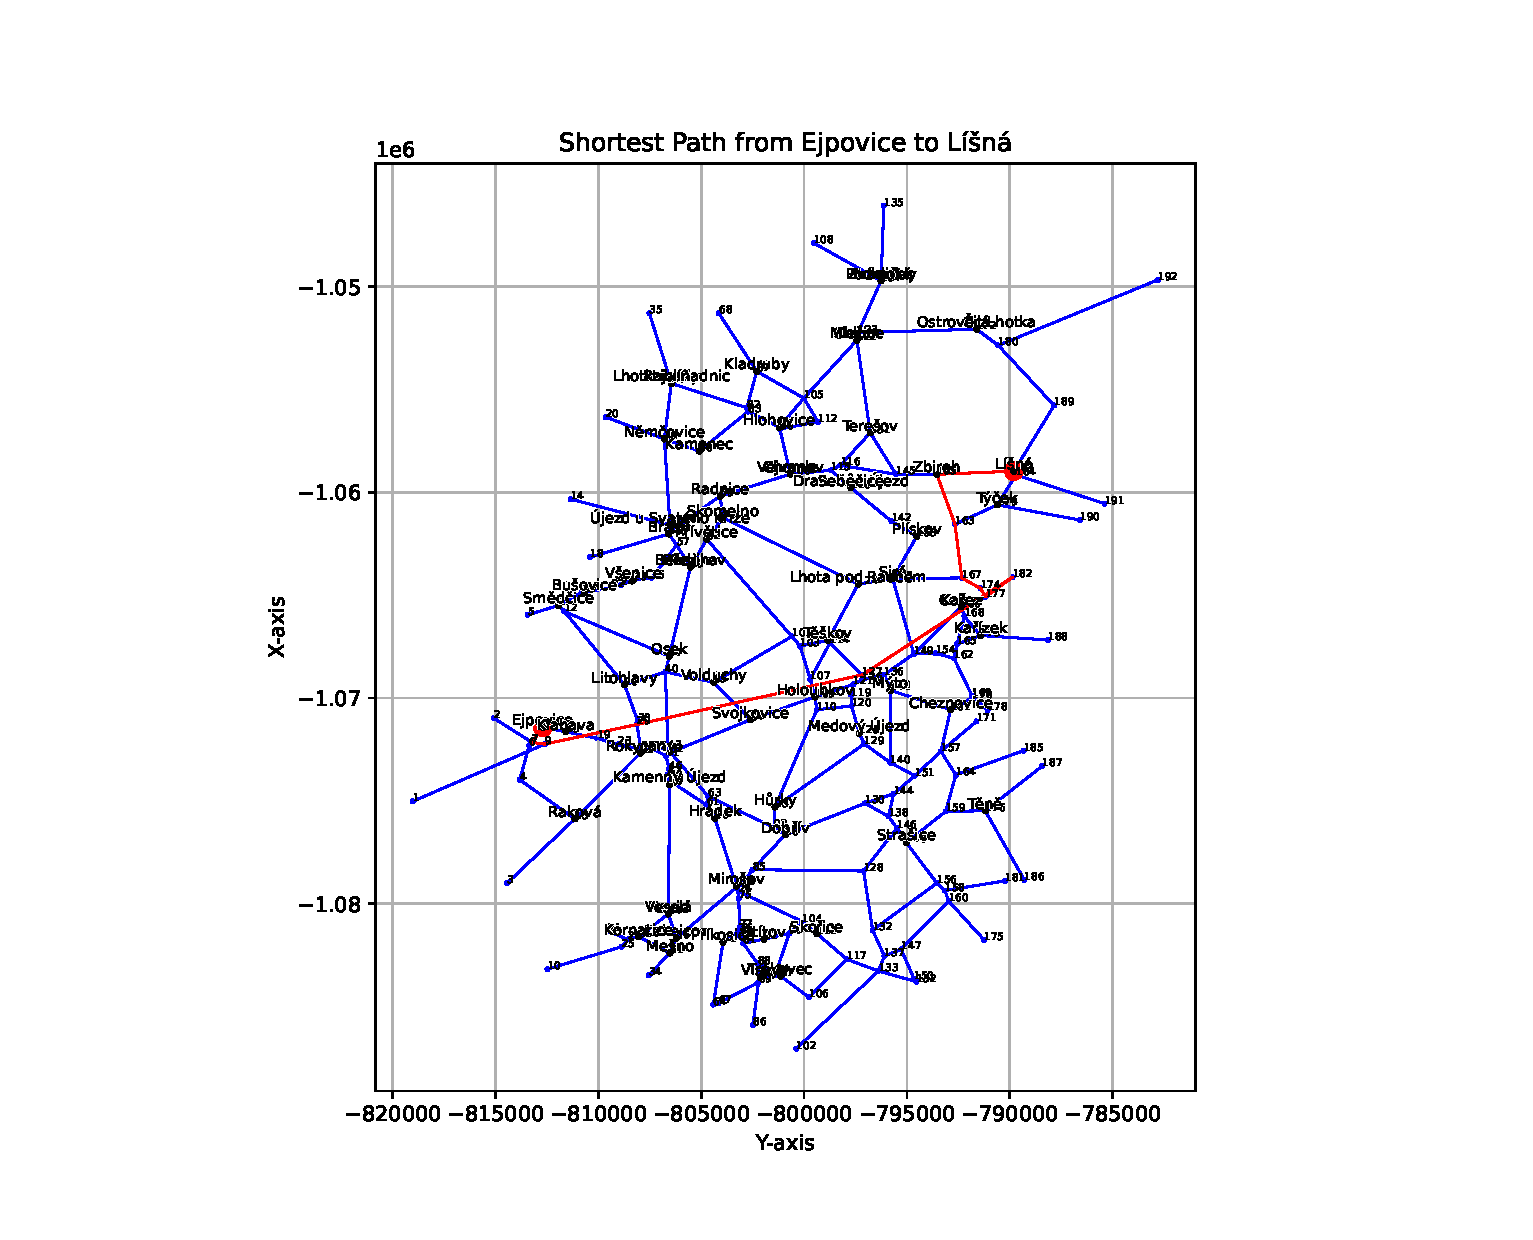
\includegraphics[width=\textwidth]{images/Ejpovice_speed_weight.eps}
    \caption{Nejkratší cesta v ohodnoceném grafu podle návrhové rychlosti}
\end{figure}
Cesta z 8 do 183: [183, 155, 163, 167, 174, 177, 182, 127, 29, 9, 7, 8] s váhou 0.13648
\paragraph{Délka cesty:} 38,2 km
%%%%%%%%%%%%%%%%%%%%%%%%%%%%%%%%%%%%%%%%%%%%%%%%%%%%%%%%%%%%%%%%%%%%%%%%%%%%%%%%%%%%%%%%%%%%%%%%%%%%%%%%%
\subsubsection*{Ohodnocený graf podle klikatosti}
\begin{figure}[H]
    \centering
    \includegraphics[width=\textwidth]{images/Ejpovice_curvature.eps}
    \caption{Nejkratší cesta v ohodnoceném grafu podle klikatosti}
\end{figure}
Cesta z 8 do 183: [183, 155, 163, 167, 174, 177, 182, 127, 29, 9, 7, 8] s váhou 11.629
\paragraph{Délka cesty:} 38,2 km
%%%%%%%%%%%%%%%%%%%%%%%%%%%%%%%%%%%%%%%%%%%%%%%%%%%%%%%%%%%%%%%%%%%%%%%%%%%%%%%%%%%%%%%%%%%%%%%%%%%%%%%%

\subsection{Minimální kostra}

%%%%%%%%%%%%%%%%%%%%%%%%%%%%%%%%%%%%%%%%%%%%%%%%%%%%%%%%%%%%%%%%%%%%%%%%%%%%%%%
\begin{figure}[H]
    \centering
    \includegraphics[width=0.65\textwidth]{images/Figure_2.eps}
    \caption{Minimální kostra neohodnoceného grafu podle Primova algoritmu}
\end{figure}

\begin{figure}[H]
    \centering
    \includegraphics[width=0.65\textwidth]{images/Figure_3.eps}
    \caption{Minimální kostra neohodnoceného grafu podle Borůvkova algoritmu}
\end{figure}
%%%%%%%%%%%%%%%%%%%%%%%%%%%%%%%%%%%%%%%%%%%%%%%%%%%%%%%%%%%%%%%%%%%%%%%%%%%%%%%
\begin{figure}[H]
    \centering
    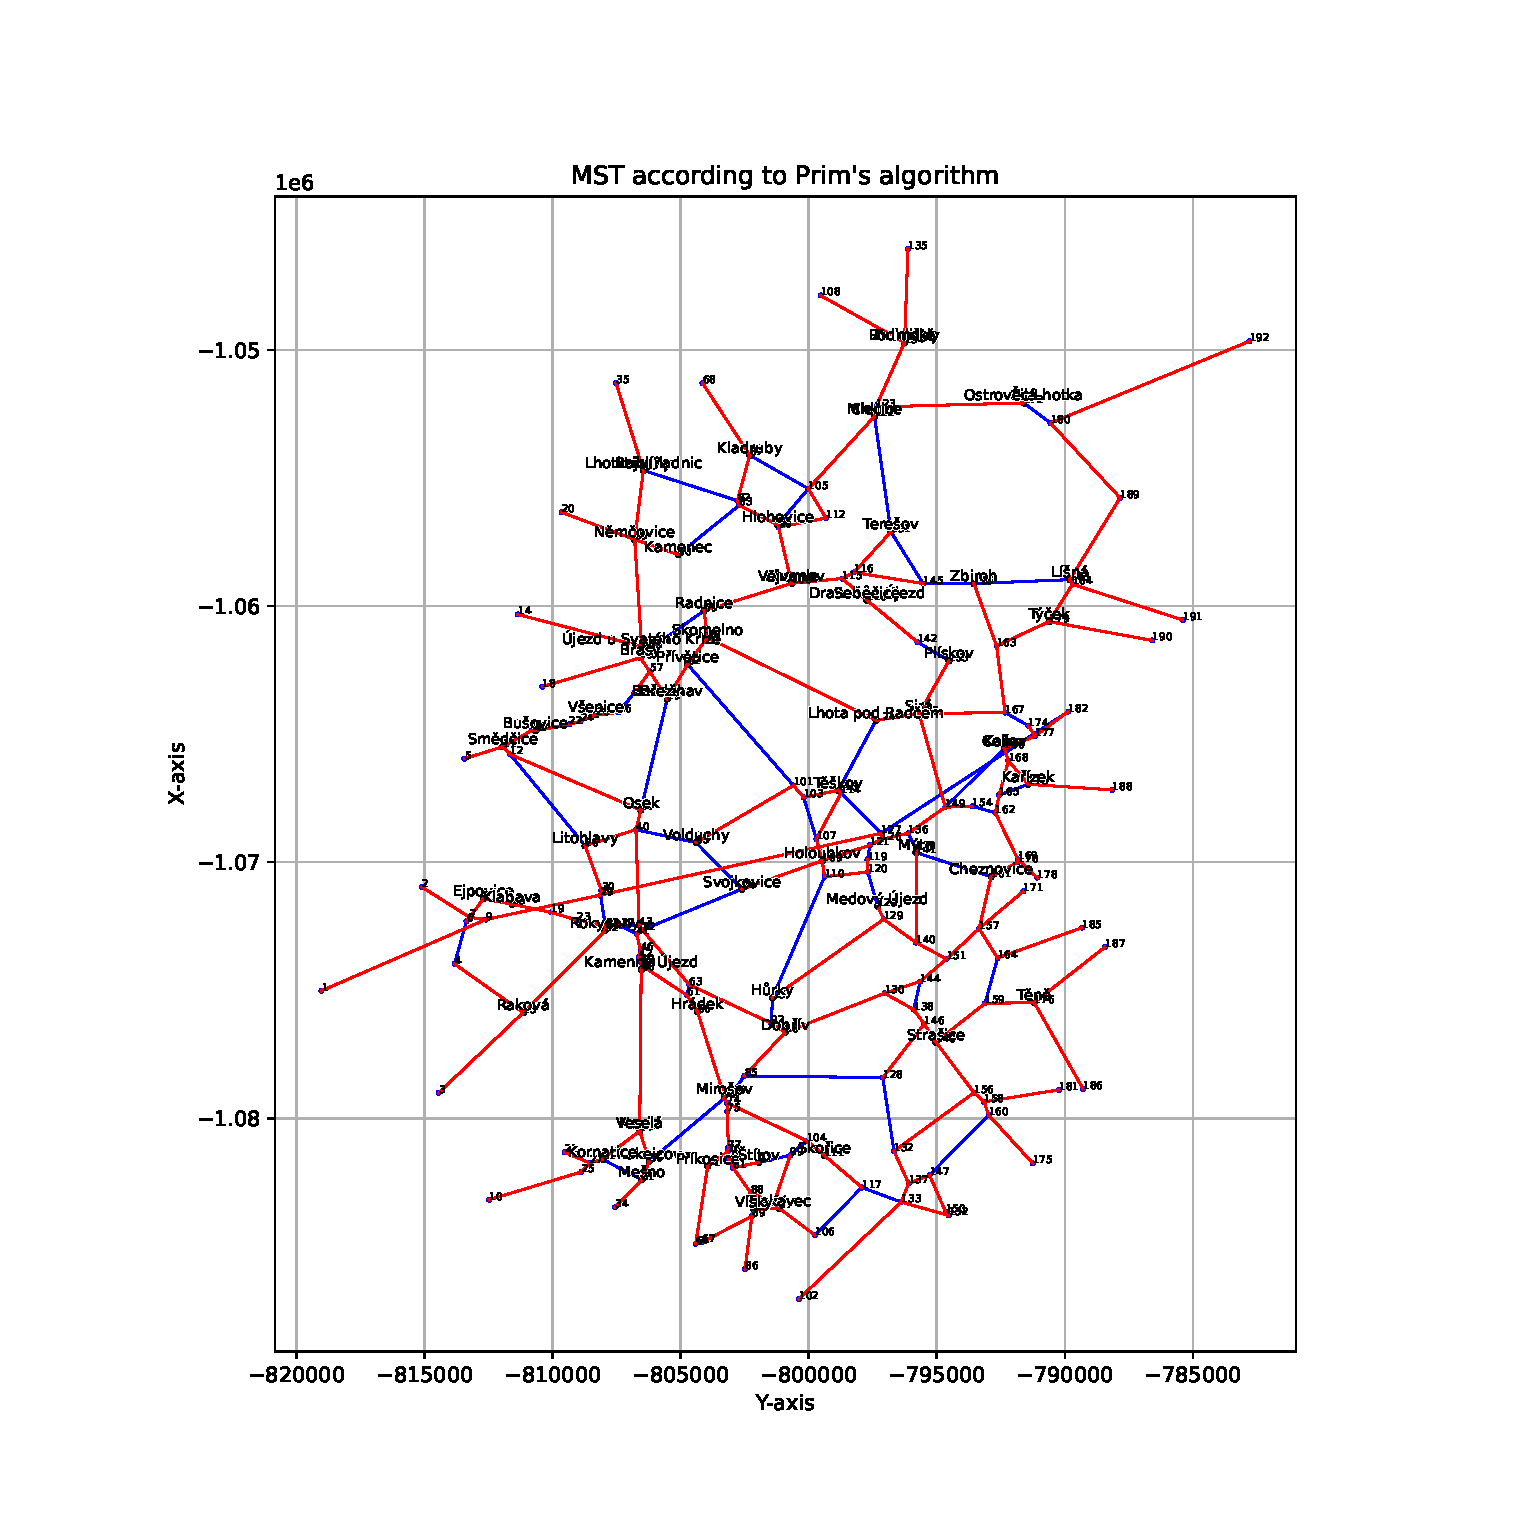
\includegraphics[width=0.65\textwidth]{images/Figure_2_curvature.eps}
    \caption{Minimální kostra v ohodnoceném grafu podle klikatosti podle Primova algoritmu}
\end{figure}

\begin{figure}[H]
    \centering
    \includegraphics[width=0.65\textwidth]{images/Figure_3_curvature.eps}
    \caption{Minimální kostra v ohodnoceném grafu podle klikatosti podle Borůvkova algoritmu}
\end{figure}
%%%%%%%%%%%%%%%%%%%%%%%%%%%%%%%%%%%%%%%%%%%%%%%%%%%%%%%%%%%%%%%%%%%%%%%%%%%%%%%
\begin{figure}[H]
    \centering
    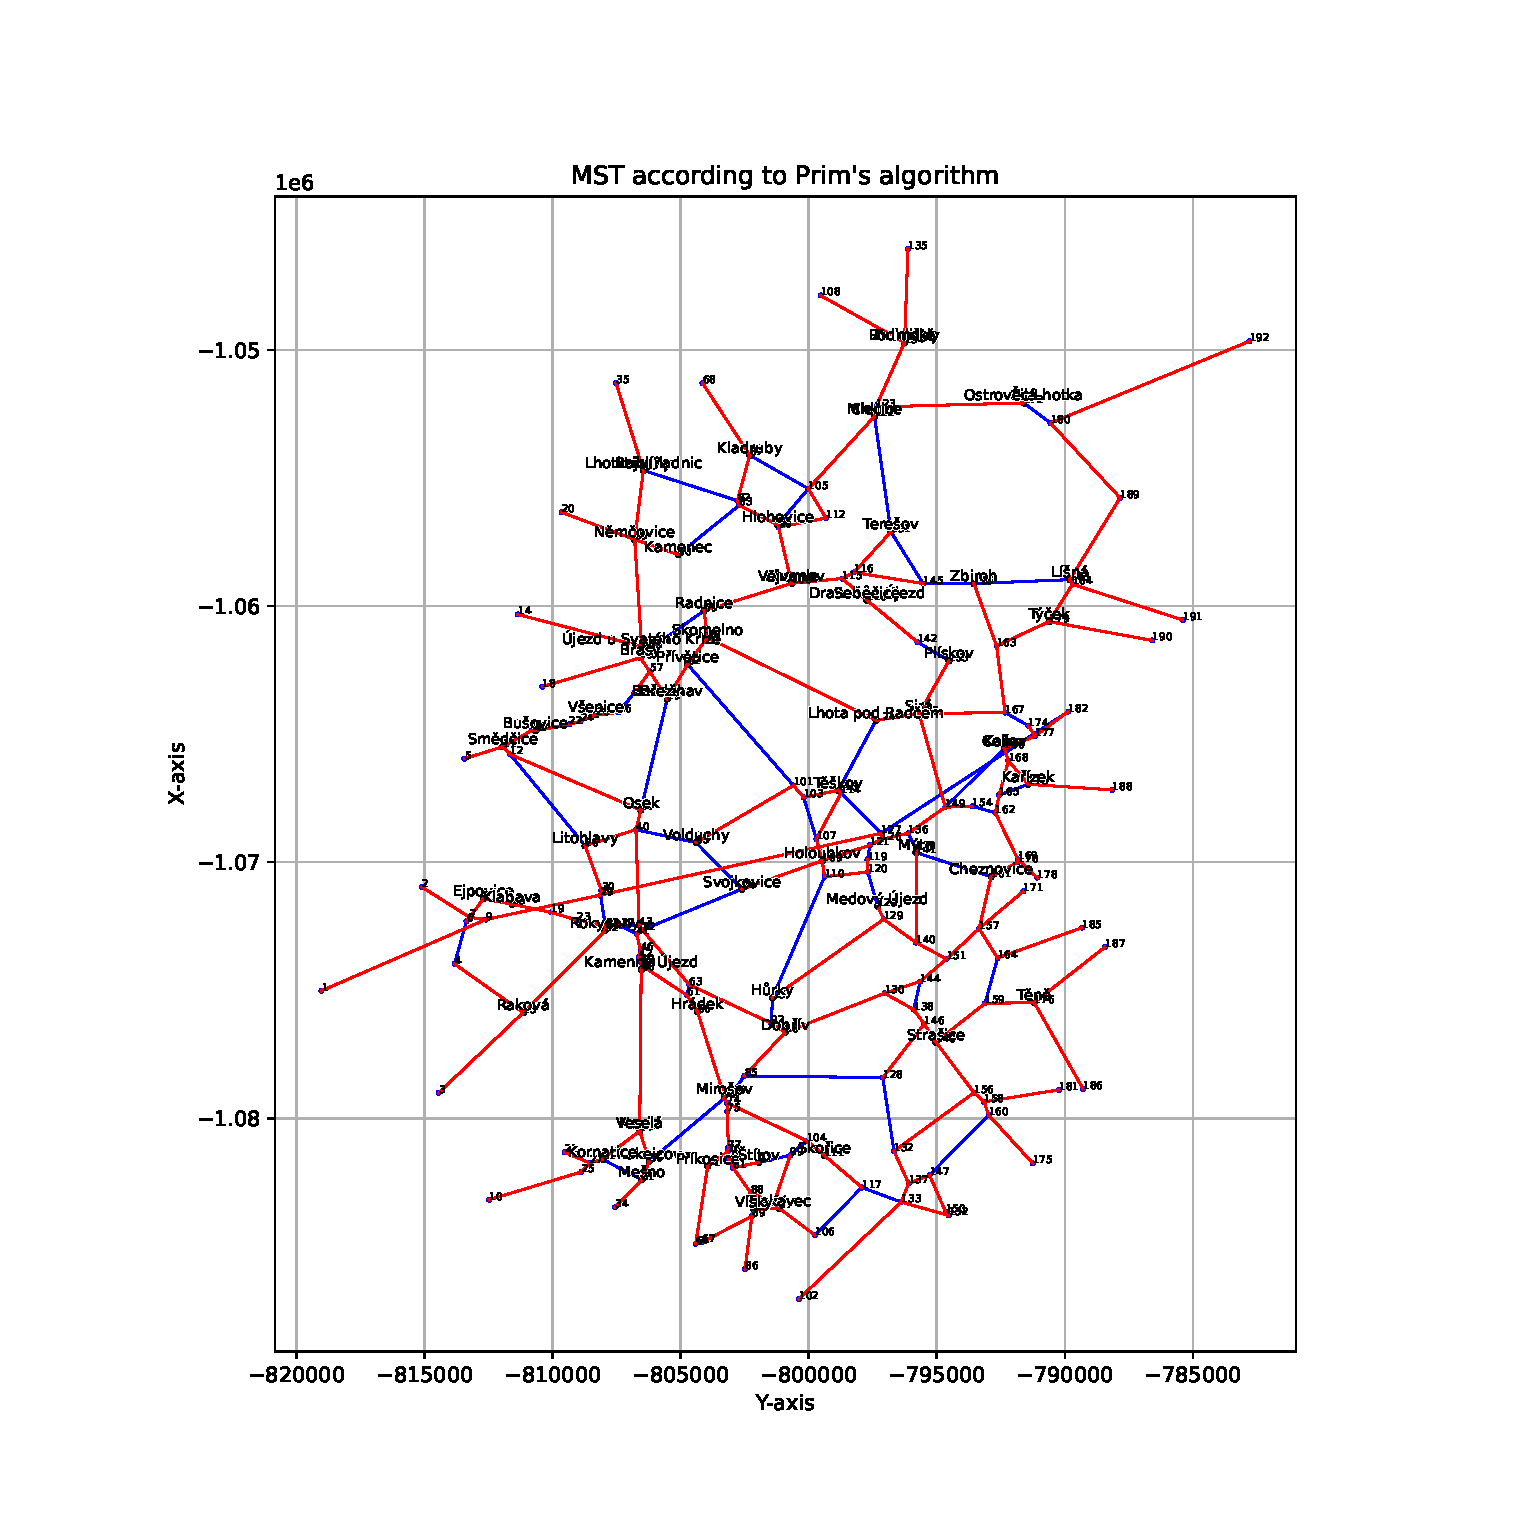
\includegraphics[width=0.65\textwidth]{images/Figure_2_curvature.eps}
    \caption{Minimální kostra v ohodnoceném grafu podle délky podle Primova algoritmu}
\end{figure}

\begin{figure}[H]
    \centering
    \includegraphics[width=0.65\textwidth]{images/Figure_3_curvature.eps}
    \caption{Minimální kostra v ohodnoceném grafu podle délky podle Borůvkova algoritmu}
\end{figure}
%%%%%%%%%%%%%%%%%%%%%%%%%%%%%%%%%%%%%%%%%%%%%%%%%%%%%%%%%%%%%%%%%%%%%%%%%%%%%%%
\begin{figure}[H]
    \centering
    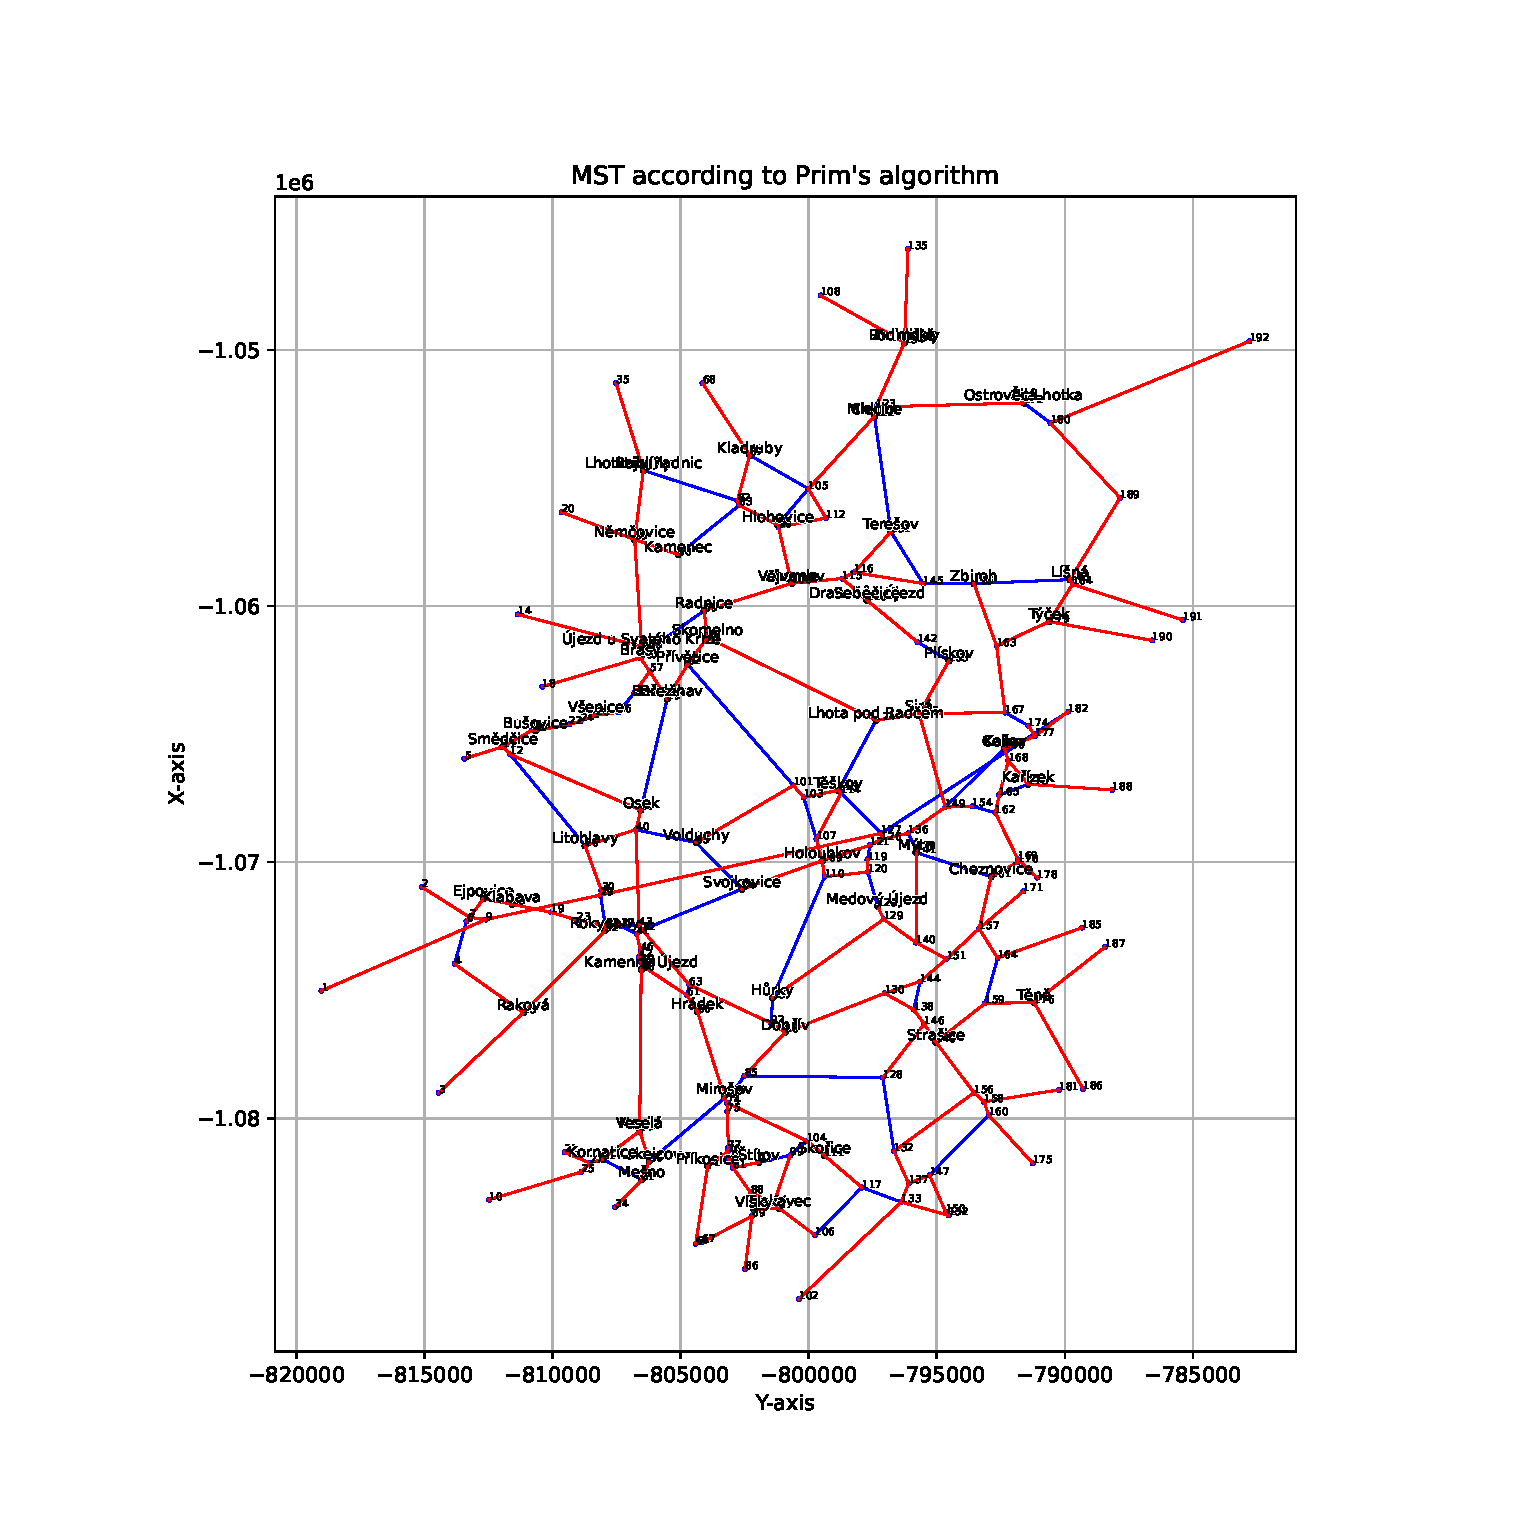
\includegraphics[width=0.65\textwidth]{images/Figure_2_curvature.eps}
    \caption{Minimální kostra v ohodnoceném grafu podle návrhové rychlosti podle Primova algoritmu}
\end{figure}

\begin{figure}[H]
    \centering
    \includegraphics[width=0.65\textwidth]{images/Figure_3_curvature.eps}
    \caption{Minimální kostra v ohodnoceném grafu podle návrhové rychlosti podle Borůvkova algoritmu}
\end{figure}